\documentclass{article}
\usepackage{graphicx}
\usepackage{amsmath}
\usepackage{enumerate}
\usepackage{amsfonts}
\usepackage[indent=20pt]{parskip}
\usepackage{mdframed}
\newmdtheoremenv{theo}{Theorem}
\numberwithin{equation}{subsection}
\numberwithin{theo}{subsection}

\begin{document}
\title{Understanding Analysis - Chapter 1}

\author{Stephen Abbott}
\maketitle

\section{The Real Numbers}
\subsection{Discussion: The Irrationality of $\sqrt{2}$}
G.H. Hardy referred to as saying that mathematics should be considered as an
art, making the suggestion that applied math isn't artistic.

Two main examples of beauty in math: (i) Euclid's proof that there are an
infinite number pf prime numbers, and (ii) that $\sqrt{2}$ is irrational. Number
two is being focused on as an example of beauty, saying it's simple and
profound.

\begin{theo}
    \label{sqtwo}
    There is no rational number whose square is $2$.
\end{theo}

\emph{Proof.} A rational number is any number that can be expressed in the form
$p/q$, where $p$ and $q$ are integers. The approach is to assume the theorem is
false and go about the argument until you reach an unacceptable conclusion, thus
leaving the theorem true because it was failed to be proven false. Start with
the assumption that there are two integers $p$ and $q$ such that:

\begin{equation}\label{irrational_proof}
    \left(\frac{p}{q}\right)^{2} = 2
\end{equation}

Goes on to do some algebra to show that $p$ and $q$ would have to be even,
meaning that the fraction in Equation \ref{irrational_proof} would be simplified by a
common factor, which is a logical impasse. 

Some discussion of how this issue persuaded the Greeks to move toward geometry
and away from arithmetic, but in modern methods this can be avoided by
strengthening the "concept of number", by moving from rational numbers to more
expanded numbers. Starting with rational numbers:

\begin{equation*}
    N = \{1,2,3,4,5,\ldots\}
\end{equation*}

Moving to integers:

\begin{equation*}
    Z = \{\ldots, -3,-2,-1,0,1,2,3,\ldots\}
\end{equation*}

Integers give you an additive identity (zero) and additive inverses necessary to
have subtraction.

For multiplication and division, $1$ is the multiplicative identity, but for
division you need multiplicative inverses.

\begin{description}
    \item[Multiplicative inverse.] The multiplicative inverse of a number is a
number that when multiplied by the original number returns $1$. Multiplicative
inverse of $a$ is $a^{-1}$. 
\end{description}

Extending the system to \emph{rational numbers}:

\begin{equation*}
    Q = \left\{\text{all fractions $\frac{p}{q}$ where $p$ and $q$ are integers
    with $q \neq 0$}\right\}
\end{equation*}

So I interpret rational numbers as including decimal numbers, which is
consistent with what I remember from elementary school. $Q$ makes up the
definition of a \emph{field}.

\begin{description}
    \item[Field.] Any set where addition and multiplication are well-defined
operations that are commutative, associative, and obey the familiar distributive
property $a(b+c) = ab + bc$. There must be an additive identity, and every
element must have an additive inverse. There must be a multiplicative identity,
and a multiplicative inverse must exist for all nonzero elements of the field.
\end{description}

Set $Q$ also has a natural order, meaning exactly one of the following is true:

\begin{equation*}
    r<s, r = s,~ \text{or} ~r > s
\end{equation*}

Can think about rational numbers as being along a number line, where for any two
rational numbers $r<s$, the rational number $(r+s)/2$ sits halfway in between.
But there is actually a hole in the number line where irrational numbers (eg,
$\sqrt{2}$) would be, even though rational numbers can approximate irrational
numbers quite well ($1.414^2 = 1.999396$). Thus, we bring in the concept of
\emph{real} numbers ($R$) in order to chain $N \subseteq Z \subseteq Q$.

Getting $R$ from $Q$ is complicated, but you're essentially patching up the
holes in $Q$ to obtain $R$. If the set of irrational numbers is $I$, then $R = Q
\cup I$. Going on to talk about the uncertainties in the relationship between
sets $I$ and $Q$. Can all irrational numbers be expressed as algebraic
combinations of \emph{n}th roots and rational numbers, or are there still other
irrational numbers beyond those of this form?


\subsection{Some Preliminaries}

We need to introduce some vocabulary from set theory and theory of functions.

\subsubsection*{Sets}

A set is a collection of objects, where objects are referred to as the
\emph{elements} of the set. In most cases, elements are real numbers, but
elements can be functions or other sets. 

Given a set $A$, we say $x \in A$ if $x$ is an element of $A$. If $x$ is not
an element of $A$ then $x \notin A$. The \emph{union} is writted $A\cup B$ and
is defined:

\begin{equation*}
    x \in A \cup B~\text{provided that}~ x \in A ~\text{or}~ x \in B ~\text{or
    potentially both}.
\end{equation*}

The \emph{intersection} $A \cap B$ is the set defined by the rule:

\begin{equation*}
    x \in A \cap B ~ \text{provided} ~ x \in A ~ \text{and} ~ x \in B
\end{equation*}

\begin{itemize}
    \item There are many ways to define a set. One example was for integers: $N
        = \{1,2,3,\ldots\}$.
    \item Sets can be described in words. Eg, $E$ is the collection of even
        natural numbers.
    \item You can provide a rule or algorithm to define a set:
        \begin{equation*}
            S = \{r \in Q: r^2 < 2\}.
        \end{equation*}
        This definition says that set $S$ contains all rational numbers whose
        squares are less than 2.
\end{itemize}

Some basic rules of sets are that (i) the union of two sets where one is a
perfect subset is equal to the larger set, and (ii) the intersection of such sets is
the smaller set. There's also the \emph{empty set}, eg: $E \cap S = \emptyset$.

\begin{description}
    \item[Empty set]. The set that contains no elements.
\end{description}

Another way of describing $E \cap S = \emptyset$ is that these sets are
\emph{disjoint}. 

\begin{description}
    \item[Inclusion relationship]. $A \subseteq B$ or $B \subseteq A$ means that
        every element of $A$ is also an element of $B$. To say $A = B$ means
        that both $A \subseteq B$ and $B \subseteq A$ are true, or that they
        contain exactly the same elements.
\end{description}


We'll want to apply union and intersection to infinite collections of sets, for
example:

\begin{align*}
    A_1 = N = \{1,2,3,\ldots\},\\
    A_2 = \{2,3,4,\ldots\},\\
    A_3 = \{3,4,5,\ldots\},
\end{align*}

and, in general, for each $n \in N$, define the set

\begin{equation*}
    A_n = \{n, n+1, n+2, \ldots\}.
\end{equation*}

The result is a nested chain of sets

\begin{equation*}
    A_1 \supseteq A_2 \supseteq A_3 \supseteq A_4 \supseteq \ldots,
\end{equation*}

where each successive set is a subset of all the previous ones. Notationally,

\begin{equation*}
    \bigcup\limits_{n=1}^\infty A_n, \bigcup\limits_{n\in N} A_n,~\text{or} ~ 
    A_1 \cup A_2 \cup A_3 \cup \ldots
\end{equation*}

So like $A_2$ is a subset of $A_1$, is how that would read. Which means the
union of all these sets is just:

\begin{equation*}
    \bigcup\limits_{n=1}^\infty A_n = A_1
\end{equation*}

Can also think about intersections stretched to infinity:

\begin{equation*}
    \bigcap\limits_{n=1}^\infty A_n = \emptyset
\end{equation*}

This one is a little weirder to think through. But yea if you shift by one for
each set as you go out to infinity, there will be no collective overlap among
all those sets.

More formally, imagine some natural number $m$ that could satisfy $m \in
\bigcap_{n=1}^\infty A_n$. This would mean that $m \in A_n$ for
\emph{every} $A_n$. But $m$ is not an element of $A_{m+1}$, so no such $m$
exists and the intersection is an empty set.

That's such nifty logic, love it.

\textbf{Set complements.} Given $A \subseteq \mathbb{R}$, the \emph{complement} of A,
written $A^c$, refers to the set of all elements of $\mathbb{R}$ not in $A$.
Thus for $A \subseteq \mathbb{R}$:

\begin{equation*}
    A^c = \{x \in \mathbb{R}: x \notin A\}.
\end{equation*}

He ends with a caution that this is an \emph{intuitive} overview of set theory.
It's been subjected to intense scrutiny over the years because it's such an
important foundation of mathematics. But, for our purposes, this level of
coverage is sufficient.

\subsubsection*{Functions}

\begin{description}
    \item[Functions.] Given two sets $A$ and $B$, a \emph{function} from $A$ to
        $B$ is a rule or mapping that takes each element $x \in A$ and
        associates it with a single element of $B$. We can write $f : A
        \rightarrow B$. Given an element $x \in A$, the expression $f(x)$ is
        used to represent the element of $B$ associated with $x$ by $f$. The set
        $A$ is called the \emph{domain} of $f$. The \emph{range} of $f$ is not
        necessarily equal to $B$ but refers to the subset of $B$ given by $\{y
        \in B : y = f(x)~ \text{for some}~x \in A\}$.
\end{description}

In the language of vectors, a function maps each each element $x \in X$ to some
$y \in Y$, although not every element in $Y$ will be mapped to from $X$.

Explaining that people used to think of functions as being strictly formulas,
but this definition of a function allows them to be far more flexible. For
example with conditional functions:

\begin{equation*}
    g(x) = 
    \begin{cases}
        1 & ~\text{if}~ x \in \mathbb{Q}\\
        0 & ~ \text{if}~ x \notin \mathbb{Q}
    \end{cases}
\end{equation*}

Domain of $g$ is all of $\mathbb{R}$, and the range is the set $\{0, 1\}$. 

Absolute value can be represented as a function, and the author argues it's a
really important one. 

\begin{equation*}
    \lvert x \rvert = 
    \begin{cases}
        x & ~\text{if} ~ x \geq 0 \\
        -x & ~\text{if} ~ x < 0
    \end{cases}
\end{equation*}

It satisfies the following important properties:

\begin{enumerate}[(i)]
    \item $\lvert ab \rvert = \lvert a \rvert \lvert b \rvert ~ \text{and} $
    \item $\lvert a + b \rvert \leq \lvert a \rvert + \lvert b \rvert$
\end{enumerate}

Says property (ii) is referred to as the \emph{triangle inequality}. Then he
proceeds with the following, which I don't quite understand. He says given three
real numbers $a$, $b$, $c$, we certainly have:

\begin{equation*}
    \lvert a-b \rvert = \lvert (a-c) + (c-b) \rvert
\end{equation*}

By the triangle inequality,

\begin{equation*}
    \lvert (a-c) + (c-b) \rvert \leq \lvert a-c \rvert + \lvert c-b \rvert
\end{equation*}

so we get

\begin{equation*}
    \lvert a-b \rvert \leq \lvert a-c \rvert + \lvert c-b \rvert
\end{equation*}

Goes on to say that $\lvert a-b \rvert = \lvert b-a \rvert$, which can be
thought of as the distance on the real number line between points $a$ and $b$,
which makes sense.

\subsubsection*{Logic and Proofs}

Writing proofs takes practice, and has a bit of an artistic quality. It's a set
of directions which should leave the reader absolutely convinced of the truth of
the proposition in question. Each step should follow logically from the previous
step or follow some agreed-upon set of facts. The steps must fit together
logically to form a cogent argument. 

He says that what we used to prove Theorem \ref{sqtwo} (ie, the irrationality
of $\sqrt{2}$) was a powerful technique called \emph{proof by contradiction}.
I guess this is considered to be an \emph{indirect} proof, and it's bad form to
use an indirect proof when a direct proof is available). An indirect proof
always starts by negating that which it's trying to prove, which can be tricky.
The argument proceeds until some logical contradiction with some accepted fact
is uncovered. 

Illustrating a few of these points with the following:

\begin{theo}
    \label{realnumequal}
    Two real numbers $a$ and $b$ are equal if and only if for every real number
    $\epsilon > 0$ it follows that $\lvert a-b \rvert < \epsilon$.
\end{theo}

\emph{Proof.} Two phrases here warrant special attention. Key in on the most
extreme phrases: \emph{for every} and \emph{if and only if}. Saying "if and only
if" implies a bidirectional relationship, ie, the proposition must be true in
both directions.

($\Rightarrow$) \emph{If $a=b$, then for every real number $\epsilon > 0$ it
follows that $\lvert a-b \rvert < \epsilon$.}

($\Leftarrow$) \emph{If for every real number $\epsilon > 0$ it follows that
    $\lvert a-b \rvert < \epsilon$, then we must have $a=b$.}

The first one is straightforward because $\lvert a-b \rvert = 0$ and it will be
less than any $\epsilon > 0$.

For the proof of the second direction, start by asserting the opposite, which is
$a \neq b$. To wrestle with this we look at the phrase "for every $\epsilon >
0$". We can pick a random value ($\epsilon_0$), \underline{and reckon that it will be equal
to $\lvert a-b \rvert$}, which is greater than zero. Ie,

\begin{equation*}
    \epsilon_0 = \lvert a-b \rvert > 0
\end{equation*}

But $\lvert a-b \rvert$ can't be simultaneously equal to \emph{and} larger than
$\epsilon$, therefore the theorem fails on its own terms and we reject the
initial assumption.

* Not sure I follow the underlined move.

He's stressing the importance of being able to manipulate the phrases "for all"
and "there exists" when dealing with proofs.

\subsubsection*{Induction}

Saying induction is used in conjunction with the natural numbers $\mathbb{N}$ or
sometimes $\mathbb{N} \cup \{0\}$. The fundamental principle of induction is
that if $S$ is a subset of $\mathbb{N}$ with properties:

\begin{enumerate}[(i)]
    \item $S$ contains 1 and
    \item whenever $S$ contains a natural number $n$, it also contains $n + 1$,
\end{enumerate}

then it must be that $S = \mathbb{N}$. 

This seems obvious to me and strange how this could be considered to be the
"fundamental principle" of induction. He says this principle can be used to
define sequences of objects and prove facts about them.

\textbf{Example.} Let $x_1 = 1$, and for each $n \in \mathbb{N}$ define

\begin{equation*}
    x_{n+1} = (1/2)x_n + 1.
\end{equation*}

Thus, $x_2 = (1/2)(1) + 1 = 3/2, x_3 = 7/4$, which leads to a definition of
$x_n$ for all $n \in \mathbb{N}$. Now, use induction to prove that

\begin{equation*}
    x_n \leq x_{n+1}
\end{equation*}

for all values of $n \in \mathbb{N}$. We've shown that this holds for $x_1$ and
$x_2$. He says that

\begin{equation*}
    \text{\emph{if} we have } x_n \leq x_{n+1}~\text{, then it follows that }
    x_{n+1} \leq x_{n+2}
\end{equation*}

I don't really understand this leap. I guess satisfying this would show that the
hypothesis hold out to infinity? But where one comes up with this from is
unclear.

We have shown $1 \in S$, we now want to show that if $x \in S$, then $n + 1 \in
S$ as well. \emph{My note.} I guess I'm starting to understand the purpose of
$S$. Through concrete examples, we build a set of $S$, which is a subset of
$\mathbb{N}$. Showing that $S$ includes more and more elements of $\mathbb{N}$,
we slowly grow evidence in favor of that hypothesis. If we can scale to $S =
\mathbb{N}$, then we know the hypothesis holds for all natural numbers. It
really is induction in the sense that you're kind of inferring some rule or
hypothesis is true based on "observations".

He goes on to say: starting from the induction hypothesis $x_n \leq x_{n+1}$, we
can multiply across the inequality by $1/2$ and add $1$ to get

\begin{equation*}
    \frac{1}{2}x_n + 1 \leq \frac{1}{2} x_{n+1} + 1.
\end{equation*}

which is precisely the desired conclusion $x_{n+1} \leq x_{x+2}$. By induction,
the claim is proved for all $n \in \mathbb{N}$.

Okay this I don't understand at all. Where in the heck does $1/2$ come from? No
idea and it's not explained at all.

An important thing to note, we're not actually using induction to prove the
original example $x_{n+1} = (1/2)x_n + 1$, we're using it to prove one property
of this equation, which is $x_n \leq x_{n+1}$ for all $n \in \mathbb{N}$.


\subsubsection*{Exercises}

\begin{enumerate}
    \item 
        \begin{enumerate}
            \item Prove that $\sqrt{3}$ is irrational. Does a similar argument
                work to show $\sqrt{6}$ is irrational?
            
\emph{Solution.} Well, if $\sqrt{3}$ is irrational, that means that $\sqrt{3}
\notin \mathbb{R}$. We can try to prove by contradiction, by asserting that
$\sqrt{3} \in \mathbb{R}$. This must mean that we should be able to find two
integers, $p$ and $q$, where

\begin{equation*}
    \left(\frac{p}{q}\right)^2 = 3
\end{equation*}

Some manipulation gets us to

\begin{align*}
    \frac{p^2}{q^2} = 3\\
    p^2 = 3q^2
\end{align*}

In the opening proof, the author uses this last line to assert that $p^2$ is a
multiple of $3$, but I'm having trouble seeing that.

Okay okay I think I'm seeing it. Take the actual case of the opening proof (ie,
prooving irrationality of $\sqrt{2}$)


\begin{equation*}
    p^2 = 2q^2
\end{equation*}

One way to think about this is that $p^2$ \emph{is} $q^2$ times $2$. Since $p$
and $q$ are integers, $p^2$ must be divisible by $2$.

So coming back to the present exercise, we can tell $p^2$ is a multiple of $3$.
But now I feel like we're going to deviate from the example, because knowing
that $p^2$ is a multiple of $3$ doesn't tell us whether $p^2$ is odd or even.

Okay, peeked at the solution. He jumps right from $p^2 = 3q^2$ to $p = 3r$,
because if a perfect square is a multiple of three then its square root must
also be a multiple of three (had to think about this one). So now we can
substitute in $3r$

\begin{align*}
    (3r)^2 = 3q^2\\
    9r^2 = 3q^2\\
    3r^2 = q^2
\end{align*}

And now we see that $q^2$ is also a multiple of $3$, meaning $q$ is a multiple
of $3$, meaning $p/q$ doesn't hold because they share a common factor.
    

            \item Where does the proof of Theorem \ref{sqtwo} break down if we
                try to use it to prove $\sqrt{4}$ is irrational?

Okay so we propose there must be two integers such that 

\begin{align}
    \left(\frac{p}{q}\right)^2 = 4\\
    \frac{p^2}{q^2} = 4\\
    p^2 = 4q^2\\
    p = 4r \label{eq1}\\
    (4r)^2 = 4q^2\\
    16r^2 = 4q^2\\
    4r^2 = q^2
\end{align}

So I don't know, it looks like the same logic is used to show that both $p$ and
$q$ are multiples of $4$ and should be able to be simplified.

Oh okay in the solution says the problem is with (\ref{eq1}), knowing a perfect
square is a multiple of $4$ doesn't tell you whether the square root is a
multiple of $4$.
    

        \end{enumerate}

    \item Show that there is no rational number $r$ satisfying $2^r$ = 3.

Go back to the definition of rational numbers and propose that $r = p/q$ where
$p$ and $q$ are integers

\begin{equation*}
    2^{\frac{p}{q}} = 3
\end{equation*}

What do I do here? Take the $p/q$ root of $2$? 

Did some digging on fractional exponents, it looks like

\begin{equation*}
    X^{p/q} = \sqrt[q]{X^p}
\end{equation*}

So then

\begin{align*}
    \sqrt[q]{2^p} = 3\\
    2^p = 3^q
\end{align*}

The solution says that, if $p > 0$, then $q > 0$, which gives $3|2^p$, which is
impossible.

I understand $3|2^p$ as $3$ dividing \emph{into} $2^p$ evenly, which I guess is
impossible. Also I'm not seeing the jump between $2^p = 3^q$ to $3|2^p$. I'm
tempted to say divide both sides by $3$, but that doesn't make any sense.

Same logic for when $p < 0$.

\item Decide which of the following represent true statements about the nature
    of sets. For any that are false, provide a specific example where the
    statement in question does not hold

    \begin{enumerate}
        \item If $A_1 \supseteq A_2 \supseteq A_3 \supseteq A_4 \cdots$ are all
            sets containing an infinite number of elements, then the
            intersection $\bigcap_{n=1}^\infty A_n$ is infinite as well.

            Example in the sets segment of the chapter looks at this. It's
            false. Imagine some element $m$ that could actually satisfy $m \in
            \bigcap_{n=1}^{\infty} A_n$. It would mean $m \in A_n$ for
            \emph{every} $A_n$, but $m \notin A_{m+1}$.

        \item If $A_1 \supseteq A_2 \supseteq A_3 \supseteq A_4 \cdots$ are all
            finite, nonempty sets of real numbers, then the intersection
            $\bigcap_{n=1}^\infty A_n$ is finite and nonempty.

            I think this is true. The intersection can't be larger than $A_1$,
            which is a finite, non empty set, and it can't be smaller than $A_n$
            which is also finite and non empty. (Solution says true).

        \item $A \cap (B \cup C) = (A \cap B) \cup C$.
            
            My hunch is this is false because the left side of the equation
            captures $A \cap C$ whereas the right doesn't... ? Solution says
            false and does so by proposing examples of sets $A$, $B$, $C$, and
            demonstrating that the equation doesn't hold.

        \item $A \cap (B \cap C) = (A \cap B) \cap C$.

        True. I think intersections are associative? Three intersections are
        three intersections, doesn't matter what order you take them in. 

        \item $A \cap (B \cup C) = (A \cap B) \cup (A \cap C)$.

        Solution says true. I can kind of visualize it. You're taking the $A$
        piece out of $B$ and $C$. This equality says it doesn't matter whether
        you take that piece out after putting $B$ and $C$ together or not.

    \end{enumerate}

    \item Produce an infinite collection of sets $A_1, A_2, A_3, \cdots$ with
        the property that every $A_i$ has an infinite number of elements, $A_i
        \cap A_j = \emptyset$ for all $i \neq j$, and $\bigcup_{i=1}^\infty A_i
        = N$.

        I really don't see this one, it feels like a paradox. If each set has an
        infinite number of elements, how could the intersection between each set
        be empty?

        Yea so solution says you just group up $N$ essentially in infinite ways,
        where each group is disjoint. Yea idk like group infinity in infinite
        ways, okay I guess.

    \item Let $A$ and $B$ be subsets of $\mathbb{R}$.

        \begin{enumerate}

            \item If $x \in (A \cap B)^c$, explain why $x \in A^c \cup B^c$.
                This shows that $(A \cap B)^c \subseteq A^c \cup B^c$.

            De Morgan's Laws once again are: 
            \begin{align*}
                (A \cap B)^c = A^c \cup B^c\\
                (A \cup B)^c = A^c \cap B^c
            \end{align*}

            So these definitions answer this problem pretty straightforwardly I
            think.

            Looked up the solution yesterday and trying this again today from memory.

            If $x \in (A \cap B)^c$, then $x \notin A \cap B$, meaning that at
            least one of the following must be true: $x \notin A$ or $x \notin
            B$. Which means either $x \in A^c$ or $x \in B^c$, which means $x
            \in A^c \cup B^c$.  

        \item Prove the reverse inclusion $(A \cap B)^c \supseteq A^c \cup B^c$,
            and conclude that $(A \cap B)^c = A^c \cup B^c$.

           Let's try just using the logic above going the other way. So if some
           element $x \in A^c \cup B^c$, that means that either $x \in A^c$ or
           $x \in B^c$, meaning that either $x \notin A$ or $x \notin B$,
           meaning that $x \notin A \cap B$, meaning that $x \in (A \cap B)^c$.


        \item Show $(A \cup B)^c = A^c \cap B^c$ by demonstrating inclusion both
            ways.

            \textbf{Going forward.} If $x \in (A \cup B)^c$, then both $x \notin
            A$ and $x \notin B$ are true, which means that $x \in A^c$ and $x
            \in B^c$, meaning that $x \in A^c \cap B^c$.

            \textbf{Going backwards.} If $x \in A^c \cap B^c$, then $x \in A^c$
            and $x \in B^c$, which means that $x \notin A \cup B$, meaning that
            $x \in (A \cup B)^c$.

        \end{enumerate}

        \begin{enumerate}
            \item Verify the triangle inequality in the special case where $a$
                and $b$ have the same sign.

                Triangle inequality again is $\lvert a + b \rvert \leq \lvert a
                \rvert + \lvert b \rvert$.

                So it's pretty clear to me that if $a$ and $b$ are both positive
                that the sides will be equal. If negative, it's definitely
                possible for the left to be less than the right. Not sure how to
                "verify" this.

                Okay, for positive, solution says $\lvert a \rvert = a$ and
                $\lvert b \rvert = b$, thus $\lvert a + b \rvert = a + b =
                \lvert a \rvert + \lvert b \rvert$.

                So for negative, the right hand still reduces to $\lvert a
                \rvert + \lvert b \rvert = a + b$. I'm pretty sure the left also
                reduces as such, adding two negatives is a negative number whose
                absolute value is equal to the sum of if those numbers were
                positive. Ie, $\lvert -a - b \rvert = \lvert a + b \rvert = a +
                b = \lvert a \rvert + \lvert b \rvert$.

                Okay so the solution uses notation like if $a < 0$, then $-a$
                would be positive. So they say, $\lvert a + b \rvert = -(a + b)
                = -a-b = \lvert a \rvert + \lvert b \rvert$.

        \end{enumerate}

    \item Given a function $f$ and a subset $A$ of its domain, let $f(A)$ represent the
        range of $f$ over the set $A$; that is, $f(A) = \{f(x) : x \in A\}$.

        \begin{enumerate}
            \item Let $f(x) = x^2$. If $A = [0, 2]$ (the closed interval $~\{x
                \in \mathbb{R} : 0 \leq x \leq 2 \}$) and $B = [1, 4]$, find
                $f(A)$ and $f(B)$. Does $f(A \cap B) = f(A) \cap f(B)$ in this
                case? Does $f(A \cup B) = f(A) \cup f(B)$? 

            I plotted this out in R, and I think the answer to the first
            question is 'yes'. 

            \begin{figure}[ht!]
                \centering
                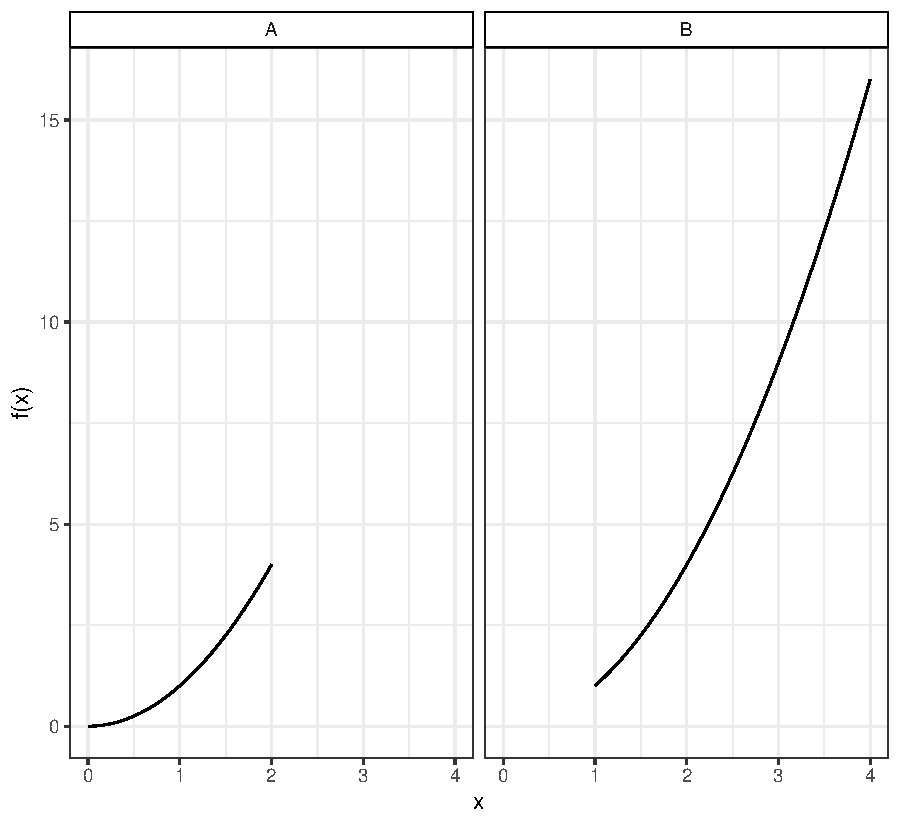
\includegraphics[width=2.5in, scale=0.5]{exercise1-2-7.pdf}
            \end{figure}

            $A \cap B = [1,2]$, $f([1,2])$ is roughly between 1 and 5, and so
           is the range of both $f(A)$ and $f(B)$. Well not $f(B)$, but it has
           the intersection with $f(A)$ that makes it work. And $f(A \cup B) =
           f(A) \cup f(B) = [0, 16]$.

       \item Find two sets $A$ and $B$ for which $f(A \cap B) \neq f(A) \cap
           f(B)$.

           Had to look at solutions. The answer is to capitalize on the fact
           that the function is $f(x) = x^2$, by $A = [-4, 0],~B = [0,
           4],~f(A\cap B) = {0},~f(A) \cap f(B) = [0, 16]$.

        \end{enumerate}


\end{enumerate}



\end{document}
